\documentclass[11pt]{article}
\usepackage[T1]{fontenc}
\usepackage[utf8]{inputenc}
\usepackage{lmodern}
\usepackage[margin=1in]{geometry}
\usepackage{amsmath,amssymb}
\usepackage{booktabs}
\usepackage{graphicx}
\usepackage{caption}
\usepackage{natbib}
\usepackage[colorlinks=true,linkcolor=blue,citecolor=blue,urlcolor=blue]{hyperref}
\graphicspath{{../figures/}}
\captionsetup{font=small,labelfont=bf}
\newcommand{\HL}{h_{1/2}}

\title{Does Faster Mean Reversion Predict Pairs-Trading Profits?\\[4pt]
\large Half-Life Evidence from a Replication of Gatev, Goetzmann and Rouwenhorst (2006)\\on Point-in-Time S\&P~500 Data, 2000--2025}
\author{Saksham Garg}
\date{October 2026 \\ \small Working paper. Code, data documentation and all results: \url{https://github.com/sakshamg251206/mean-reversion-half-life}; archived at \href{https://doi.org/10.5281/zenodo.23157543}{doi:10.5281/zenodo.23157543}.}

\begin{document}
\maketitle

\begin{abstract}
\noindent
We replicate the distance-based pairs-trading rule of \citet{gatev2006} (GGR) on daily point-in-time S\&P~500 constituents from 1999 to 2025, and ask whether the \emph{mean-reversion half-life} of a pair's spread, estimated only from formation-period data, predicts the pair's out-of-sample trading return. The replication confirms the well-documented decay of the strategy: the top-20 portfolio earns 0.24\% per month gross on committed capital in 2000--2012 (Newey--West $t=2.21$) and 0.00\% in 2013--2025 ($t=-0.01$), against 0.81\% per month in GGR's 1962--2002 sample. In the 2000--2012 development sample, formation half-life is a strong cross-sectional predictor: pairs in the fastest-reverting quintile out-earn the slowest quintile by 1.74\% per six-month trading period ($t=3.29$), and the Fama--MacBeth slope on the half-life rank is $-0.021$ ($t=-3.29$), robust to controlling for the distance rank. However, half-life is barely persistent (Spearman correlation between formation and realised trading-period half-life 0.03), and in a pre-specified holdout (2013--2025, parameters frozen and committed before evaluation) the effect shrinks to 0.36\% ($t=1.04$, $p=0.30$); a half-life-filtered portfolio chosen on the development sample does not beat plain GGR, and no hypothesis survives a Holm adjustment. Net of 10~bp per leg-side, neither strategy is profitable after 2012. Sub-period analysis shows that the half-life premium decayed gradually after 2010 rather than being a crisis artefact. We conclude that estimated half-life captured a real but transient source of pairs profits, and that its in-sample predictive power is not evidence of a deployable signal.
\end{abstract}

\section{Introduction}

Pairs trading is the canonical relative-value strategy: find two securities whose prices have moved together, short the relatively expensive one and buy the cheap one when they diverge, and unwind when they converge. \citet{gatev2006} turned this practitioner heuristic into a transparent, testable rule and documented annualised excess returns of roughly 11\% on CRSP stocks over 1962--2002. A large follow-up literature has shown that these profits have declined \citep{dofaff2010,dofaff2012} and that alternative selection rules---cointegration, copulas, stochastic spread models---perform differently \citep{elliott2005,avellaneda2010,rad2016,krauss2017}.

A pair trade is a bet on mean reversion. The natural measure of how fast a spread mean-reverts is its \emph{half-life}: under an Ornstein--Uhlenbeck (OU) model the expected time for a deviation to halve. Practitioner texts recommend selecting or sizing pairs by half-life \citep{vidyamurthy2004,chan2013}, the implicit claim being that pairs which reverted quickly in the past will revert quickly---and therefore profitably---in the future. GGR's selection criterion, the sum of squared differences (SSD) between normalised prices, does not use the speed of reversion at all. Whether half-life adds out-of-sample information is an empirical question that, to our knowledge, has not been tested with a strict development/holdout protocol.

This paper makes three contributions, which we label explicitly throughout:
\begin{enumerate}
\item \textbf{Replication.} We re-implement GGR's rule exactly (12-month formation, 6-month trading, 2$\sigma$ entry, exit on crossing, six overlapping portfolios, committed and employed capital, wait-one-day execution) on point-in-time S\&P~500 constituents for 2000--2025---an out-of-sample test of GGR itself.
\item \textbf{Extension.} We estimate half-lives for every selected spread with four estimators (OLS AR(1), Kendall bias-corrected, exact OU maximum likelihood, and a model-free crossing interval), three lookbacks and two spread definitions; characterise their stationarity and cointegration properties; and implement a cointegration/OU trading rule whose holding period is scaled by half-life.
\item \textbf{Original research.} We test whether formation half-life predicts trading-period returns (quintile sorts and Fama--MacBeth regressions), whether half-life is persistent, and whether a half-life filter improves GGR---with parameters chosen on 2000--2012 only, frozen in a version-controlled file, and evaluated once on 2013--2025, with multiple-testing adjustments.
\end{enumerate}

The answer is a clear negative result with an informative in-sample pattern. Half-life ``works'' in the development sample with $t$-statistics above 3, survives costs there, and passes a deflated-Sharpe check against the 21 variants tried. It does not hold up out of sample. The development-sample evidence alone would have been publishable; the holdout shows why it should not be believed without one.

\section{Literature}

\textbf{Distance-based pairs trading.} \citet{gatev2006} match stocks by minimum SSD between cumulative total-return indices and trade divergences beyond two formation-period standard deviations. They report top-20 excess returns of 1.44\% per month on employed capital and 0.81\% on committed capital (no waiting), falling to 0.90\% and 0.52\% with one-day-delayed execution, profits concentrated before 1989, low exposure to standard risk factors, and returns that random pairs do not reproduce. \citet{dofaff2010} extend the sample and document a secular decline in profitability, and \citet{dofaff2012} show that after realistic commissions and market impact much of the post-2002 profit disappears.

\textbf{Model-based approaches.} Cointegration \citep{englegranger1987,johansen1991} provides the formal justification for spread trading \citep{vidyamurthy2004}. \citet{elliott2005} model the spread as a mean-reverting Gaussian Markov chain observed in noise; \citet{avellaneda2010} model residual returns as OU processes and trade $s$-scores. \citet{rad2016} compare distance, cointegration and copula methods on US data and find similar performance for distance and cointegration. \citet{krauss2017} surveys the field.

\textbf{Mean reversion and reversal.} Short-horizon reversal \citep{jegadeesh1990,lehmann1990} and medium-horizon momentum \citep{jegadeeshtitman1993} are the known return patterns that pairs trading could be repackaging. GGR show that random pairs do not earn their returns, so pairs profits are not simple reversal.

\textbf{Statistical methodology.} Half-lives follow from the OU process \citep{uhlenbeck1930}; AR(1) coefficients are biased downward in finite samples \citep{kendall1954}, so naive half-life estimates are too short. Unit-root and stationarity tests \citep{dickeyfuller1979,kpss1992} and variance ratios \citep{lomackinlay1988} characterise spreads. We use Newey--West standard errors \citep{neweywest1987}, Fama--MacBeth regressions \citep{famamacbeth1973}, and guard against data snooping with Holm and Benjamini--Hochberg adjustments \citep{holm1979,bh1995} and the deflated Sharpe ratio \citep{bailey2014}, following the concerns raised by \citet{harvey2016}. Survivorship bias in historical samples is analysed in \citet{brown1992}.

\section{Hypotheses}

All hypotheses were written down before any results were inspected (design specification in the repository, \texttt{docs/superpowers/specs/}). Significance is 5\%, two-sided.
\begin{description}
\item[H1 (replication).] GGR excess returns are positive in 2000--2025 and smaller than in 1962--2002.
\item[H2 (core).] Shorter formation-period half-life predicts higher trading-period pair returns (negative slope).
\item[H3.] Formation half-life is positively correlated with the half-life realised in the trading period.
\item[H4.] Any H2 advantage survives realistic transaction costs.
\item[H5.] SSD selection combined with a half-life filter beats SSD selection alone on the 2013--2025 holdout.
\end{description}

\section{Data}

\textbf{Universe.} Point-in-time S\&P~500 membership comes from dated constituent snapshots (the public \texttt{fja05680/sp500} dataset, 1996--2026). On each formation date the universe is the set of index members on the first formation day with no missing price in the 12-month formation window---the closest analogue to GGR's ``no day without a trade'' screen. Stocks are \emph{not} required to survive the trading period; a position in a stock that stops trading is closed at the last available price, as in GGR.

\textbf{Prices.} Daily split- and dividend-adjusted closes from Yahoo Finance serve as cumulative total-return indices, 1999-01-01 to 2025-12-31. Of the 1,117 tickers that were ever members in the window, Yahoo returns data for 691; the remaining 426 have been deleted after delisting (acquisitions, bankruptcies, take-privates). Three cleaning rules address free-data pathologies: (i) a ticker's prices are kept only within its membership spells plus 18 months (the longest horizon any portfolio needs), which removes history belonging to unrelated firms that later re-used the ticker; (ii) interior gaps of at most five days are forward-filled, gaps after a stock's last price never; (iii) 11 tickers with more than 10\% zero daily returns---illiquid securities Yahoo serves under re-used symbols---are dropped. 618 tickers remain. SPY and the VIX index come from the same source, NBER recession dates from FRED, and GICS sectors from the current constituent list.

\textbf{Survivorship.} Figure~\ref{fig:coverage} shows the share of each year's members with complete prices: 44\% in 1999, 52\% in 2005, 64\% in 2010, 70\% in 2013, 86\% in 2020 and 97\% in 2025. Missing firms are disproportionately those later acquired or failed---precisely the pairs in which one leg jumps or collapses and a convergence trade loses. The bias therefore most likely inflates pairs returns, and does so mainly in the development sample. The average formation universe contains 339 stocks (Table~\ref{tab:tradestats}).

\begin{figure}[t]\centering
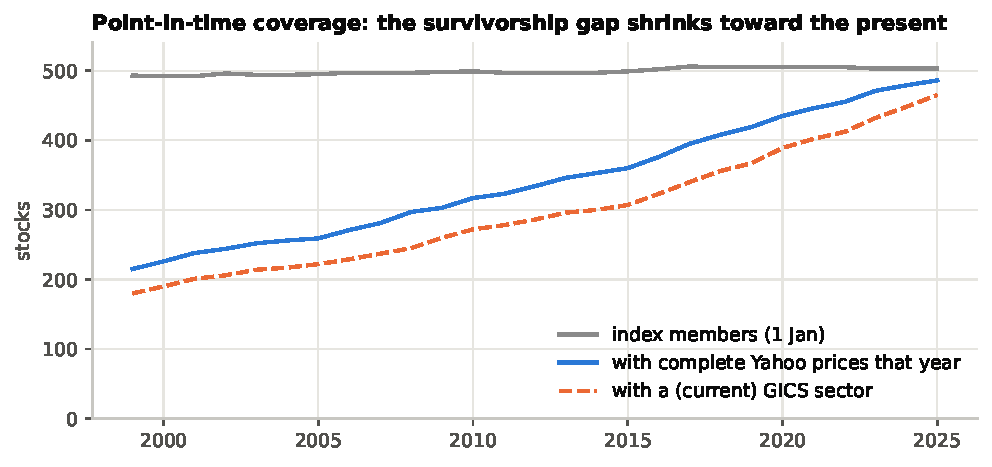
\includegraphics[width=0.8\textwidth]{fig01_coverage.pdf}
\caption{Point-in-time coverage. Grey: index members on 1 January; blue: members with a complete Yahoo price history that year; orange: members with a (current) GICS sector. The gap is the residual survivorship bias of free data.}
\label{fig:coverage}
\end{figure}

\section{Methodology}

\subsection{Pair formation and trading (GGR)}
For stock $i$ let $P^i_t=\prod_{s\le t}(1+r^i_s)$ be the cumulative total-return index rebased to one on the first formation day. For every pair in the universe,
\begin{equation}
D_{ij}=\sum_{t\in\mathcal F}(P^i_t-P^j_t)^2 ,
\end{equation}
computed for all pairs at once from the Gram matrix. Portfolios hold the $N\in\{5,20\}$ lowest-$D$ pairs, a sector-restricted top-20 (survivor-conditioned; see Limitations), and 20 random pairs (seeded) as a baseline. During the six-month trading window, prices remain normalised to the formation start (as in GGR's Figure~1). A position opens at the close when $|P^i_t-P^j_t|>2\hat\sigma_{ij}$, where $\hat\sigma_{ij}$ is the formation-period standard deviation of the difference; it is \$1 long the lower and \$1 short the higher stock. It closes when the prices cross, when a leg stops trading (at its last price), or on the last trading day; pairs may re-open. In the wait-one-day variant every order executes at the next close.

\textbf{Returns.} Inside a trade, legs are buy-and-hold, so the daily payoff per dollar committed is $\pi_t=s\,(a_{t-1}r^i_t-b_{t-1}r^j_t)$ with leg values $a,b$ compounding from one and $s=\pm1$. The \emph{committed-capital} return divides the portfolio payoff by the number of pairs selected; the \emph{employed-capital} return divides by the number of pairs with an open position that day (GGR's eq.~(2); the only definition consistent with their Table~1). Daily returns are compounded within months and averaged across the up to six overlapping portfolios started one month apart. Trading starts at the first trading day of each month from January 2000 to July 2025: 307 portfolios.

\textbf{Costs.} A cost of $c$ basis points per leg per side is charged on every open and close, so a round trip costs $4c$ per pair. We report $c\in[0,40]$ and use $c=10$~bp as the headline net figure.

\subsection{Half-life}
Let $S_t$ be the spread. The OU process $dS_t=\kappa(\theta-S_t)\,dt+\sigma\,dW_t$ has the exact daily discretisation
\begin{equation}
S_{t+1}=\theta(1-\phi)+\phi S_t+\varepsilon_{t+1},\qquad \phi=e^{-\kappa},
\end{equation}
so a deviation is expected to decay as $\phi^h$ and halves after
\begin{equation}
\HL=\frac{\ln 2}{\kappa}=-\frac{\ln 2}{\ln\phi}.
\end{equation}
$\phi\ge1$ implies no reversion ($\HL=\infty$); $\phi\le0$ an oscillating process (undefined). The interpretation assumes a linear, Gaussian, constant-parameter process; real spreads violate all three, which is why persistence (H3) is tested rather than assumed. Estimators, all computed on formation data only:
\begin{enumerate}
\item \emph{OLS}: regress $S_t$ on $S_{t-1}$ with intercept, lookbacks of 63, 126 and 252 days.
\item \emph{Kendall-corrected}: $\tilde\phi=\hat\phi+(1+3\hat\phi)/T$, removing the first-order bias $E[\hat\phi]-\phi\approx-(1+3\phi)/T$ \citep{kendall1954}.
\item \emph{Exact OU MLE}: the Gaussian likelihood including the stationary distribution $S_0\sim N(\theta,\sigma_\varepsilon^2/(1-\phi^2))$ of the first observation (conditional MLE coincides with OLS).
\item \emph{Crossing interval}: mean days between sign changes of the demeaned spread (model-free).
\end{enumerate}
Spreads are GGR's normalised-price difference and, as a check, the log spread $\log p^i_t-\beta\log p^j_t$ with $\beta$ from formation OLS. Unit tests verify that each estimator recovers a known half-life on simulated OU paths and that the Kendall correction reduces small-sample bias.

\subsection{Diagnostics}
For every candidate pair we compute the ADF $p$-value (H$_0$ unit root), KPSS $p$-value (H$_0$ stationarity), Engle--Granger $p$-value on log prices, a Johansen trace test, and the variance ratio $VR(10)$ of the spread.

\subsection{Predictive tests}
For each formation we keep the 100 lowest-SSD pairs, giving a panel of 30,700 pair-periods.
\textbf{Quintile sorts}: within each formation, pairs are sorted into half-life quintiles; the time series of Q1 (fastest) minus Q5 (slowest) six-month returns is tested with Newey--West standard errors (six lags for the overlap). \textbf{Fama--MacBeth}: in each formation, regress pair returns on the cross-sectional percentile rank of half-life (robust to infinite half-lives), optionally with the SSD rank and the Engle--Granger $p$-value; average the slopes and use Newey--West errors.

\subsection{Validation protocol}
The 150 portfolios starting January 2000 to June 2012 form the \emph{development} sample (155 months of returns); the 151 portfolios starting from January 2013 form the \emph{holdout} (156 months); the six portfolios starting July--December 2012, whose trading periods cross the boundary, are excluded from both. (The configured cut-off, 2012-07-01, fell on a Sunday, so July 2012 belongs to the embargo.) Every parameter choice---the half-life filter (H5) and the OU holding rule---was made on the development sample only, logged with all 24 variants tried, and written to \texttt{experiments/frozen.yaml}, which was committed to version control before the holdout script ran. The holdout script refuses to run if that file or the configuration has changed, and records the commit hash with its results. Two departures from ``holdout untouched'' must be disclosed. The GGR replication (H1), which involves no choices, was computed on the full sample before the freeze. And the robustness script (Section~8) was run after the freeze but before the formal holdout script, so the holdout values in the parameter-sensitivity grid and cost curves---including those of the frozen half-life-filtered and OU strategies---were seen before Table~\ref{tab:holdout} was produced. Neither informed any parameter: all choices had already been committed.

\textbf{Look-ahead checks.} Universe membership uses the formation-start snapshot; every estimate ($\hat\sigma$, $\beta$, half-lives, test statistics) uses formation data only; a unit test perturbs all prices after date $t$ and confirms every signal and P\&L up to $t$ is unchanged; a second test perturbs trading-period prices and confirms all formation features are unchanged.

\section{Paper Replication}
\label{sec:replication}

Table~\ref{tab:replication} reports the GGR portfolios. In the development sample the top-20 portfolio earns 0.24\% per month on committed capital ($t=2.21$, annualised Sharpe 0.62), the top-5 0.19\% ($t=1.79$), the sector-restricted top-20 0.15\% ($t=1.91$) and random pairs 0.14\% ($t=0.56$) with three times the drawdown. In the holdout all four are indistinguishable from zero. Over the full period the top-20 earns 0.12\% per month ($t=1.92$) committed and 0.21\% ($t=2.12$) employed; with one-day-delayed execution, 0.10\% ($t=1.59$) and 0.16\% ($t=1.67$). For comparison, GGR report 0.81\% (committed, no wait) for 1962--2002 and 0.38\% (employed, wait one day) for 1989--2002. H1 is therefore only partly supported: returns are positive in 2000--2012 and close to GGR's late-sample level, but have vanished since 2013.

\begin{table}[t]\centering\small
\caption{GGR replication: monthly excess returns on committed capital, gross of costs, no waiting. $t$: Newey--West (6 lags). Sharpe annualised. Development sample: portfolios starting 2000-01 to 2012-06; holdout: 2013-01 to 2025-07.}
\label{tab:replication}
\begin{tabular}{llrrrrr}
\toprule
Sample & Portfolio & Mean (\%/mo) & $t$ & Sharpe & Max DD & \% months $>0$ \\
\midrule
Dev 2000--12 & Top 5 & 0.19 & 1.79 & 0.40 & $-10.4\%$ & 49.7 \\
 & Top 20 & 0.24 & 2.21 & 0.62 & $-9.7\%$ & 52.9 \\
 & Sector top 20 & 0.15 & 1.91 & 0.46 & $-8.1\%$ & 50.3 \\
 & Random 20 & 0.14 & 0.56 & 0.17 & $-29.8\%$ & 45.2 \\
 & SPY buy-and-hold & 0.23 & 0.55 & 0.18 & $-50.8\%$ & 56.1 \\
\midrule
Holdout 2013--25 & Top 5 & 0.00 & 0.06 & 0.01 & $-5.8\%$ & 51.9 \\
 & Top 20 & $-0.00$ & $-0.01$ & $-0.00$ & $-6.2\%$ & 43.6 \\
 & Sector top 20 & $-0.01$ & $-0.24$ & $-0.06$ & $-7.7\%$ & 45.5 \\
 & Random 20 & $-0.01$ & $-0.10$ & $-0.03$ & $-18.3\%$ & 49.4 \\
 & SPY buy-and-hold & 1.24 & 5.03 & 1.05 & $-23.9\%$ & 70.5 \\
\midrule
Full 2000--25 & Top 20 & 0.12 & 1.92 & 0.39 & $-9.7\%$ & 48.4 \\
 & Top 20, employed & 0.21 & 2.12 & 0.47 & & \\
 & Top 20, wait one day & 0.10 & 1.59 & 0.33 & $-9.8\%$ & \\
\bottomrule
\end{tabular}
\end{table}

\begin{table}[t]\centering\small
\caption{Trading statistics of the top-20 portfolio (analogue of GGR Table~2), full sample.}
\label{tab:tradestats}
\begin{tabular}{lr}
\toprule
Average stocks in the formation universe & 339 \\
Average pairs that open per 6-month period (of 20) & 19.4 \\
Average round trips per pair & 1.50 \\
Average entry trigger ($2\hat\sigma$, normalised price units) & 0.050 \\
Share of same-sector pairs (where sector is known) & 0.67 \\
\bottomrule
\end{tabular}
\end{table}

Trading intensity is close to GGR's (19.4 of 20 pairs open, against 19.3; 1.50 round trips per pair, against 1.96; a 5.0\% average trigger gap, against 5.3\%). Figure~\ref{fig:example} shows the mechanics for the top pair of the first development formation (Southern Co./Ameren, two utilities), and Figures~\ref{fig:equity}--\ref{fig:rolling} show cumulative returns, drawdowns and the rolling mean.

\begin{figure}[p]\centering
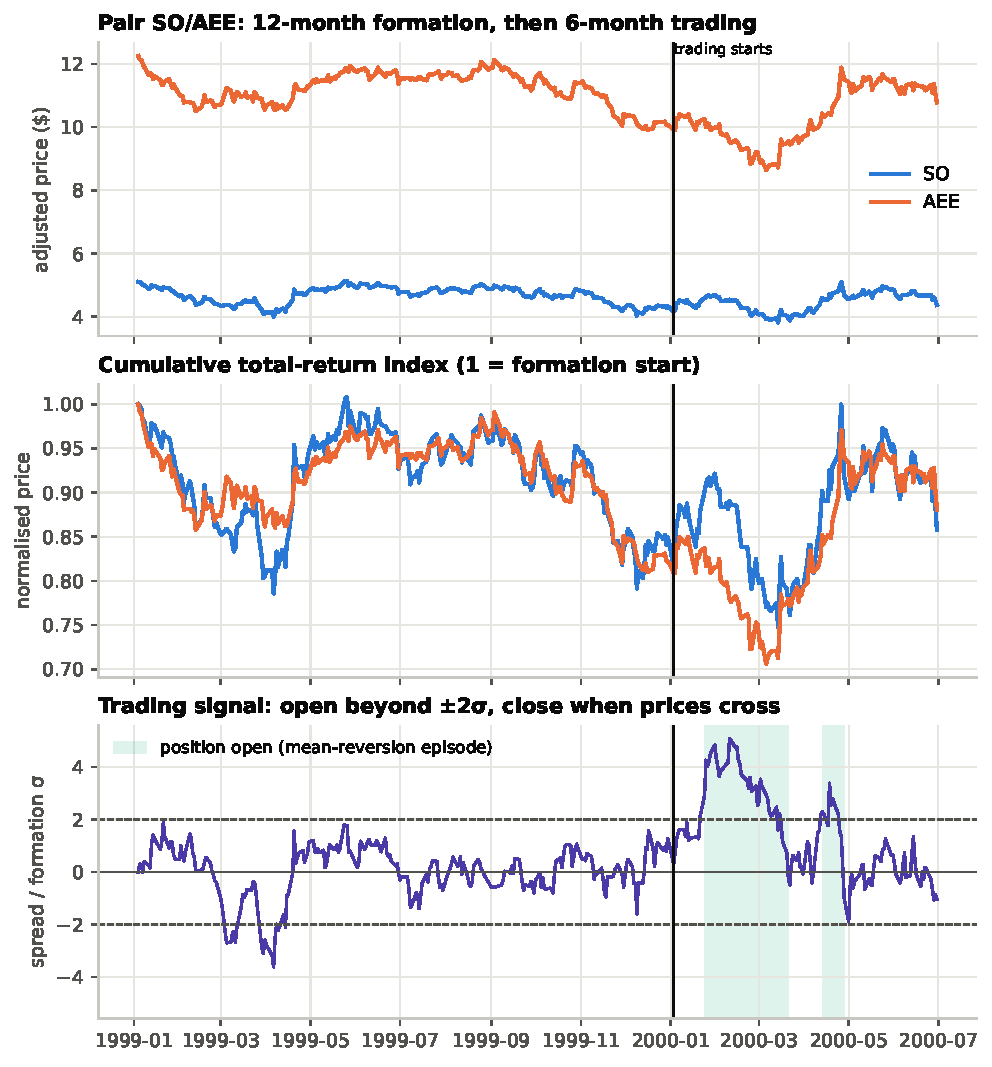
\includegraphics[width=0.82\textwidth]{fig02_example_pair.pdf}
\caption{One pair through the pipeline. Top: adjusted prices. Middle: cumulative total-return indices normalised to the formation start. Bottom: spread in formation standard deviations; shaded intervals are open positions (mean-reversion episodes). The vertical line marks the end of formation.}
\label{fig:example}
\end{figure}

\begin{figure}[t]\centering
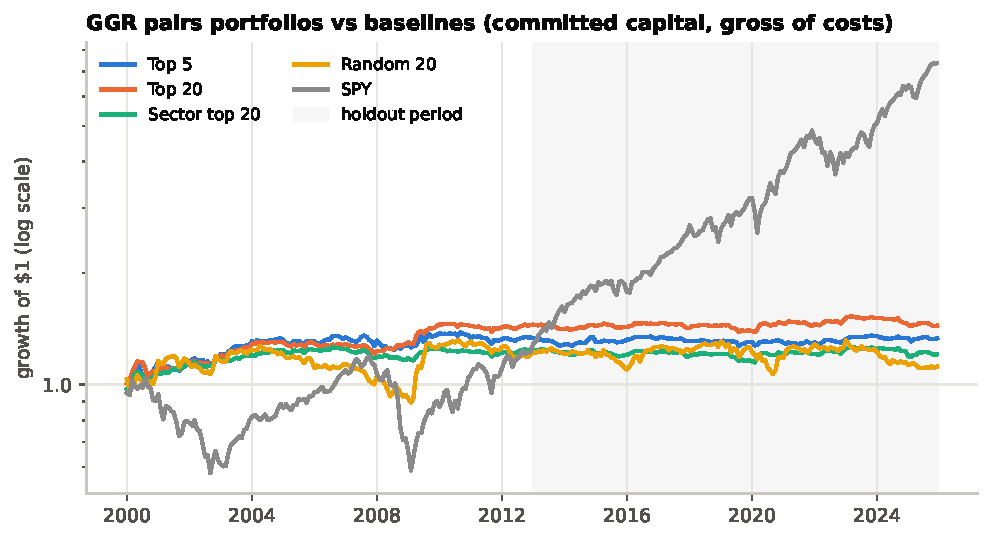
\includegraphics[width=0.85\textwidth]{fig03_equity_curves.pdf}
\caption{Growth of \$1 (log scale), committed capital, gross. Shaded: holdout period.}
\label{fig:equity}
\end{figure}

\begin{figure}[t]\centering
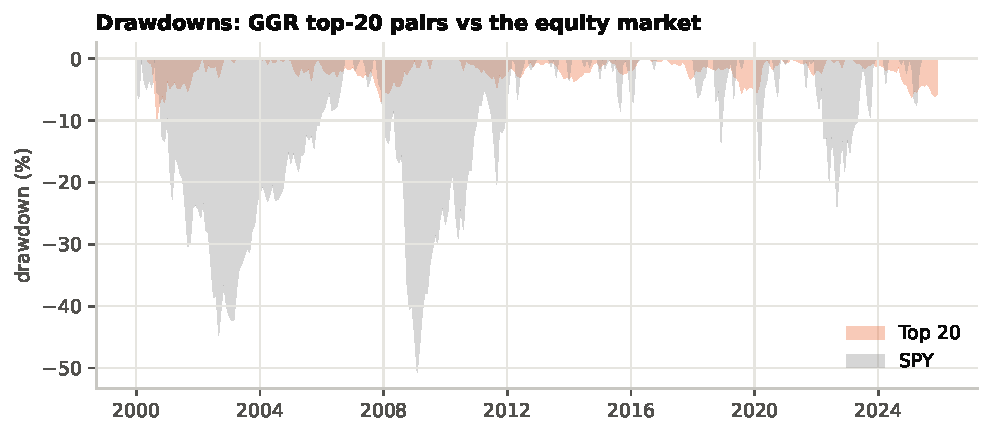
\includegraphics[width=0.49\textwidth]{fig04_drawdowns.pdf}
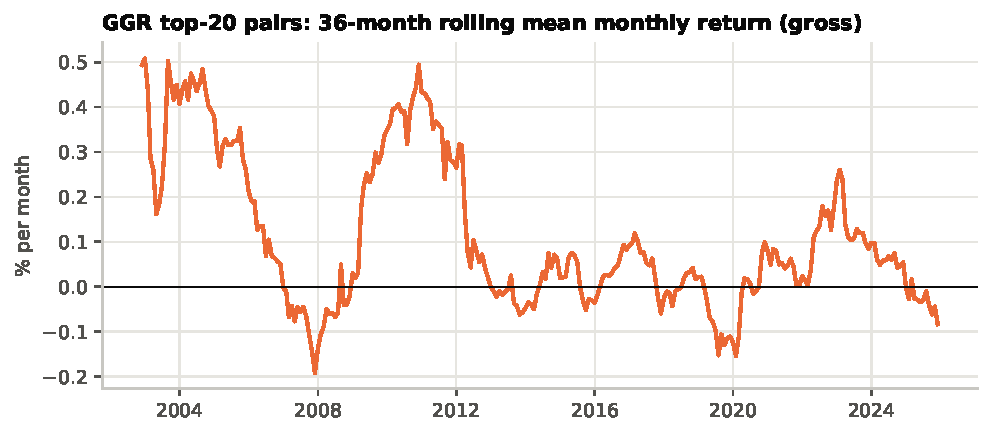
\includegraphics[width=0.49\textwidth]{fig05_rolling_performance.pdf}
\caption{Left: drawdowns of the top-20 portfolio and SPY. Right: 36-month rolling mean monthly return of the top-20 portfolio.}
\label{fig:rolling}
\end{figure}

\section{Results}

\subsection{What do the selected spreads look like?}
Formation half-lives are short and tightly distributed (Table~\ref{tab:hl}, Figure~\ref{fig:hldist}): the median OLS estimate on 252 days is 8.8 trading days, the Kendall correction raises it to 11.0 days, and the exact OU MLE gives 8.4 days. Estimators agree closely in rank (Figure~\ref{fig:agree}), except the 63-day window, which is noisier. Yet only 54\% of the top-100 spreads (61\% of the top-20) reject a unit root with ADF at 5\%, 37\% (47\%) reject no-cointegration with Engle--Granger, and 43\% fail KPSS (Figure~\ref{fig:diag}). SSD selects spreads that \emph{looked} stationary over one year; formally, about half of them are not distinguishable from random walks. The top pair in Figure~\ref{fig:example} is an example: ADF $p=0.22$, Engle--Granger $p=0.50$.

\begin{table}[t]\centering\small
\caption{Formation half-lives (trading days), development sample, top-100 SSD pairs per formation (15,000 pair-periods).}
\label{tab:hl}
\begin{tabular}{lrrrr}
\toprule
Estimator & Median & P10 & P90 & Share $\infty$ \\
\midrule
OLS, 63 days & 5.7 & 2.5 & 16.3 & 0.017 \\
OLS, 126 days & 7.7 & 3.9 & 17.4 & 0.004 \\
OLS, 252 days & 8.8 & 5.3 & 16.7 & 0.001 \\
Kendall-corrected (252) & 11.0 & 6.1 & 26.5 & 0.006 \\
OU exact MLE (252) & 8.4 & 5.2 & 15.3 & 0.001 \\
Crossing interval (252) & 8.7 & 6.3 & 14.0 & 0.000 \\
OLS, log-hedged spread & 8.0 & 4.9 & 14.6 & 0.000 \\
\midrule
Realised in trading period (OLS) & 16.2 & & & \\
\bottomrule
\end{tabular}
\end{table}

\begin{figure}[t]\centering
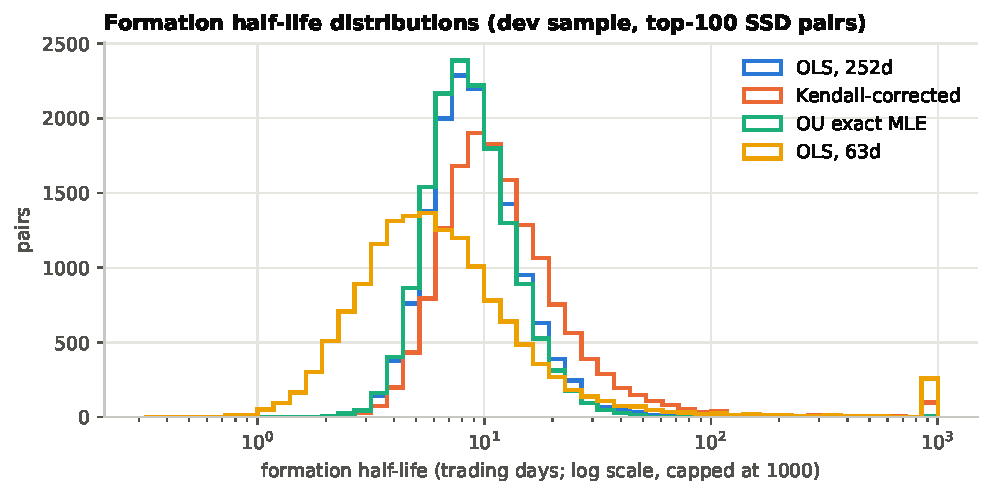
\includegraphics[width=0.49\textwidth]{fig06_halflife_distributions.pdf}
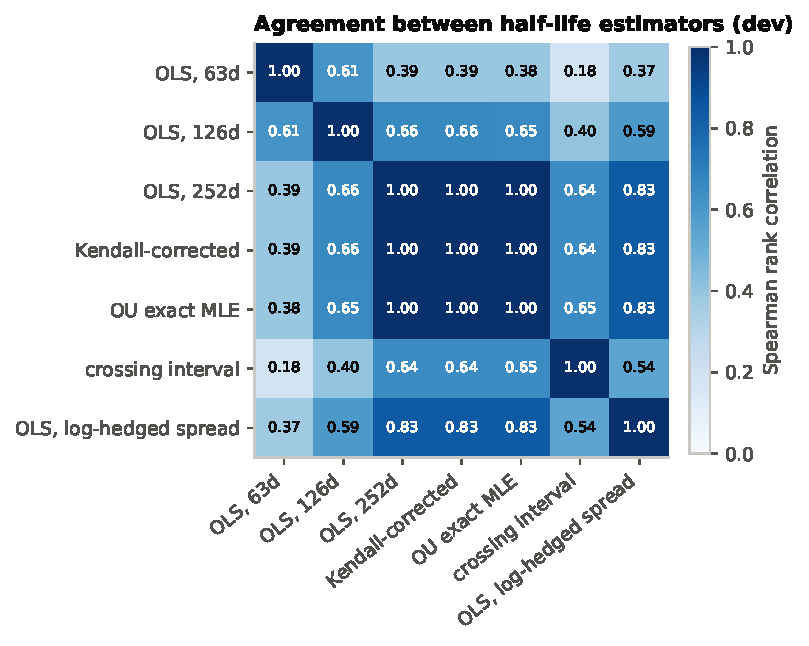
\includegraphics[width=0.43\textwidth]{fig07_estimator_agreement.pdf}
\caption{Left: distributions of formation half-life by estimator (log scale). Right: Spearman rank correlations between estimators.}
\label{fig:hldist}\label{fig:agree}
\end{figure}

\begin{figure}[t]\centering
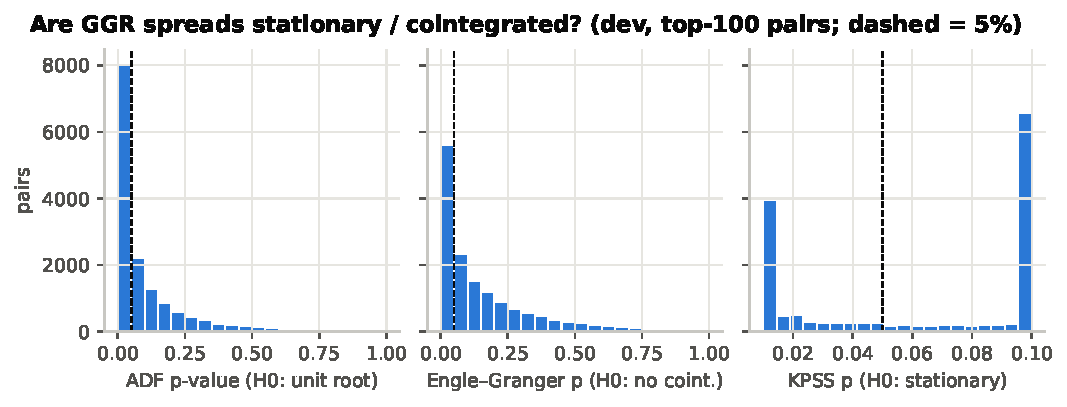
\includegraphics[width=0.9\textwidth]{fig08_diagnostics.pdf}
\caption{Stationarity and cointegration $p$-values of GGR spreads (development sample, top-100 pairs). Dashed line: 5\%.}
\label{fig:diag}
\end{figure}

\subsection{H3: is half-life persistent?}
Barely. The Spearman correlation between formation half-life (OLS, 252 days) and the half-life realised in the following six months is 0.029 in the development sample---statistically different from zero only because of the 15,000 observations---and $-0.011$ ($p=0.19$) in the holdout. The median spread reverts at half the speed after selection (8.8 versus 16.2 days), and a sizeable mass of trading-period spreads does not revert at all (Figure~\ref{fig:persist}). Figure~\ref{fig:rollinghl} shows that even the pair most often ranked first (Freddie Mac/Fannie Mae) has a 126-day rolling half-life that swings between two and several hundred days. H3 is rejected in economic terms.

\begin{figure}[t]\centering
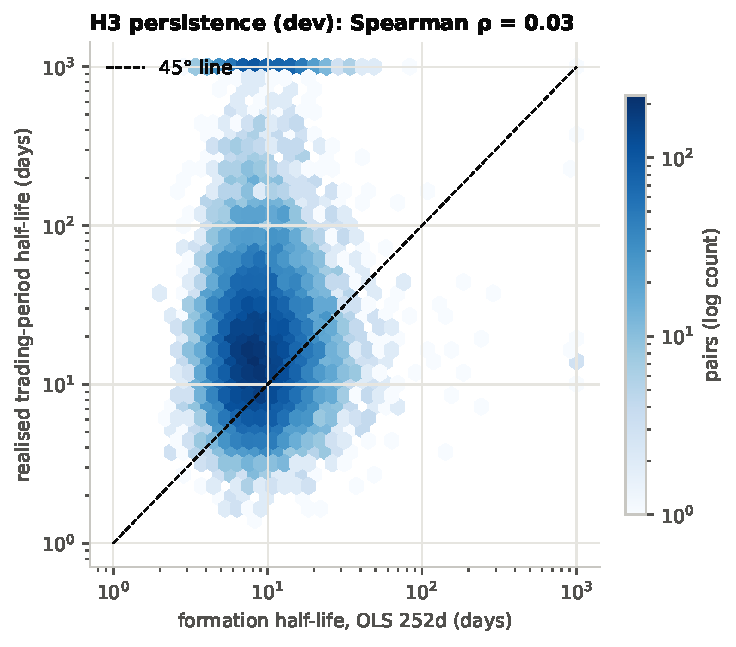
\includegraphics[width=0.45\textwidth]{fig09_persistence.pdf}
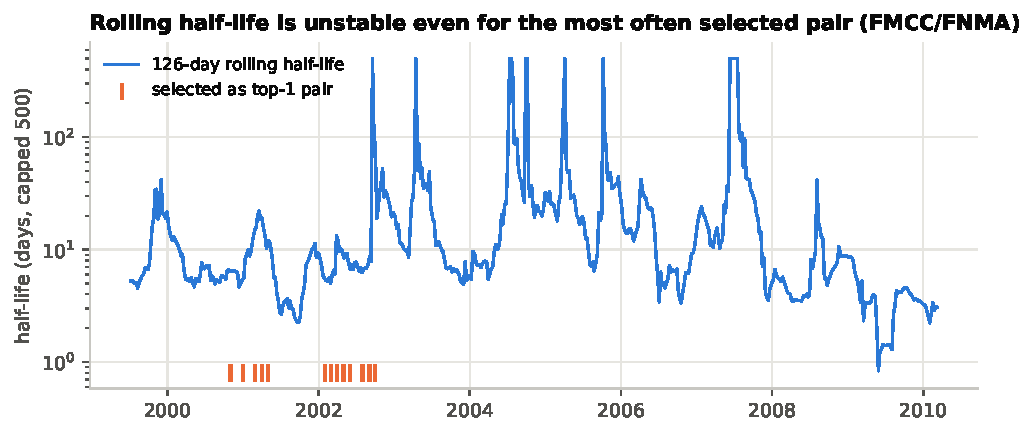
\includegraphics[width=0.53\textwidth]{fig10_rolling_halflife.pdf}
\caption{Left: formation versus realised half-life (development sample; capped at 1,000 days). Right: rolling half-life of the most frequently selected top pair.}
\label{fig:persist}\label{fig:rollinghl}
\end{figure}

\subsection{H2 in the development sample}
Despite the weak persistence, formation half-life sorts future returns strongly in 2000--2012 (Table~\ref{tab:h2dev}, Figure~\ref{fig:h2dev}). With the OLS 252-day estimator, Q1 pairs earn 2.40\% per six-month trading period and Q5 pairs 0.67\%; the spread of 1.74\% has $t=3.29$, and 1.52\% ($t=2.92$) net of 10~bp. The Kendall, OU-MLE and log-spread estimators give the same answer; the short 63-day window does not ($t=1.52$). In Fama--MacBeth regressions the half-life rank slope is $-0.021$ ($t=-3.29$), unchanged ($-0.023$, $t=-3.31$) when the SSD rank is added. Interestingly, the SSD rank enters \emph{positively} ($+0.011$, $t=2.62$): within the top 100, closer pairs do not earn more once speed is controlled for.

\begin{table}[t]\centering\small
\caption{H2, development sample: mean six-month pair return by formation half-life quintile (Q1 fastest), gross. $t$ for Q1$-$Q5, Newey--West (6 lags), 150 formations.}
\label{tab:h2dev}
\begin{tabular}{lrrrrrrr}
\toprule
Estimator & Q1 & Q2 & Q3 & Q4 & Q5 & Q1$-$Q5 & $t$ \\
\midrule
OLS, 63 days & 2.18 & 1.76 & 1.53 & 1.71 & 1.52 & 0.66 & 1.52 \\
OLS, 126 days & 2.25 & 2.08 & 1.54 & 1.79 & 1.03 & 1.22 & 2.35 \\
OLS, 252 days & 2.40 & 1.86 & 2.54 & 1.23 & 0.67 & 1.74 & 3.29 \\
Kendall-corrected & 2.41 & 1.85 & 2.55 & 1.26 & 0.62 & 1.79 & 3.31 \\
OU exact MLE & 2.44 & 1.88 & 2.58 & 1.14 & 0.64 & 1.80 & 3.26 \\
Crossing interval & 2.01 & 2.25 & 2.04 & 1.43 & 0.96 & 1.05 & 2.34 \\
OLS, log-hedged spread & 2.46 & 2.23 & 1.85 & 1.60 & 0.55 & 1.91 & 3.14 \\
\bottomrule
\end{tabular}

\vspace{6pt}
\begin{tabular}{lrrrr}
\toprule
Fama--MacBeth (dev) & (1) & (2) & (3) & \\
\midrule
HL rank (percentile) & $-0.0210$ ($-3.29$) & $-0.0226$ ($-3.31$) & & \\
log HL & & & $-0.0095$ ($-2.02$) & \\
SSD rank / 100 & & $0.0109$ ($2.62$) & $0.0103$ ($2.39$) & \\
Engle--Granger $p$ & & & $-0.0164$ ($-1.86$) & \\
\bottomrule
\end{tabular}
\end{table}

\begin{figure}[t]\centering
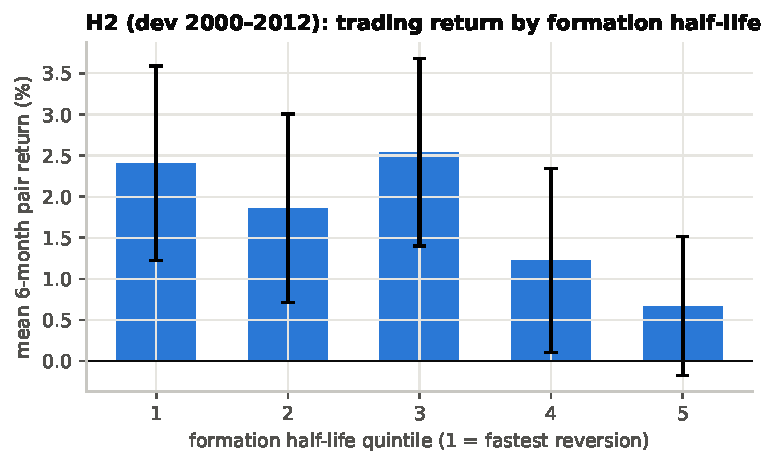
\includegraphics[width=0.49\textwidth]{fig11_h2_quintiles_dev.pdf}
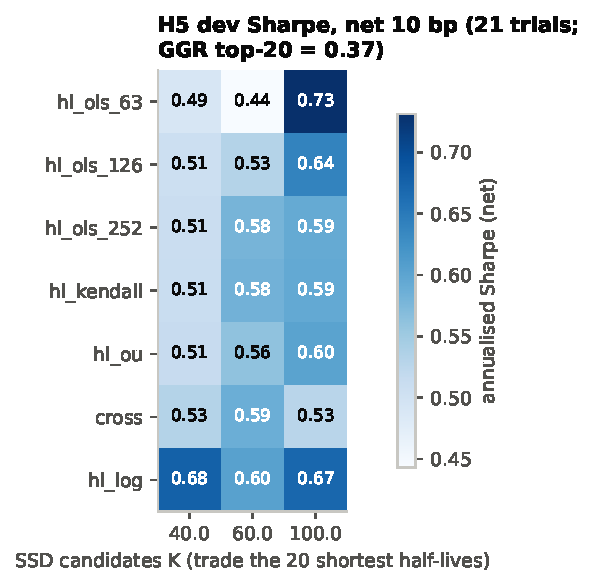
\includegraphics[width=0.49\textwidth]{fig12_h5_dev_grid.pdf}
\caption{Left: H2 in the development sample (OLS 252-day half-life; $\pm$95\% NW intervals). Right: net Sharpe ratios of the 21 half-life-filter variants tried on the development sample.}
\label{fig:h2dev}
\end{figure}

\textbf{Development-sample choices.} The H5 filter takes the $K$ lowest-SSD pairs and trades the 20 with the shortest half-life. Among 21 variants ($K\in\{40,60,100\}$ $\times$ 7 estimators) the best net-of-cost Sharpe ratio, 0.73 versus 0.37 for GGR top-20, came from $K=100$ with the 63-day OLS half-life; the deflated-Sharpe probability given 21 correlated trials is 0.99. The OU strategy (20 lowest Engle--Granger $p$-values among the top 100, $|z|>2$ entry, exit at the mean, maximum holding $m\times\HL$) had Sharpe ratios of $-1.02$, $-0.24$ and 0.12 for $m=1,2,3$; $m=3$ was frozen. These choices were committed before the holdout was run.

\section{Robustness}

\textbf{Parameters.} Varying the formation length (6 or 12 months), entry threshold ($k\in\{1.5,2,2.5\}$) and portfolio size ($N\in\{5,20,50\}$) changes magnitudes but not signs: all 18 development-sample net Sharpe ratios are positive (0.08 to 0.53), all 18 holdout ratios negative ($-0.14$ to $-0.50$; Figure~\ref{fig:sens}). The decay is not an artefact of GGR's arbitrary 12/6/2$\sigma$ choices.

\textbf{Regimes.} Net returns are concentrated in stress (Table~\ref{tab:regimes}, Figure~\ref{fig:regimes}): 0.62\% per month in 2008--09 versus 0.11\% in 2000--07, $-0.11\%$ in 2010--19 and $-0.05\%$ in 2020--25; 0.42\% in the top VIX tercile versus $-0.14\%$ and $-0.19\%$ in the others; 0.63\% in NBER recession months versus $-0.03\%$ in expansions. Regime labels are assigned ex post; this is description, not a timing rule.

\textbf{Sectors.} Utilities dominate the top-20 (2,631 of 6,140 pair-periods, as in GGR's 71\%), but earn nothing ($-0.19\%$ per six months). Profitable pairs are disproportionately cross-sector or in Financials (1.89\%) and Industrials (2.53\%) (Figure~\ref{fig:sector}). The most ``textbook'' pairs---utilities with tight, slow spreads---are not where the returns were.

\textbf{Sub-periods of H2.} Table~\ref{tab:sub} decomposes the half-life premium. It is significant in 2000--mid-2007 (1.56\%, $t=2.69$) and in the crisis (3.35\%, $t=2.27$), then falls to 0.66\% ($t=0.69$) in 2010--12 and stays near 0.35\% in both halves of the holdout. Excluding the crisis does not remove the development-sample effect (1.33\%, $t=2.66$). The premium decays over time; it is not a crisis artefact, and it was already weak in the last part of the development sample.

\begin{table}[t]\centering\small
\caption{H2 by sub-period: Q1$-$Q5 six-month return (OLS 252-day half-life), gross. Descriptive; computed after the holdout run.}
\label{tab:sub}
\begin{tabular}{lrrrr}
\toprule
Trade-start period & Formations & Q1$-$Q5 (\%) & $t$ (NW) & $p$ \\
\midrule
2000-01 -- 2007-06 & 90 & 1.56 & 2.69 & 0.007 \\
2007-07 -- 2009-12 (crisis) & 30 & 3.35 & 2.27 & 0.023 \\
2010-01 -- 2012-06 & 30 & 0.66 & 0.69 & 0.49 \\
2013-01 -- 2019-12 (holdout) & 84 & 0.38 & 0.91 & 0.37 \\
2020-01 -- 2025-07 (holdout) & 67 & 0.34 & 0.58 & 0.56 \\
\bottomrule
\end{tabular}
\end{table}

\begin{table}[t]\centering\small
\caption{GGR top-20 monthly returns by regime, net of 10 bp, full sample (\%).}
\label{tab:regimes}
\begin{tabular}{llrrr}
\toprule
Split & Regime & Mean & SD & Months \\
\midrule
Era & 2000--07 & 0.11 & 1.49 & 96 \\
 & 2008--09 & 0.62 & 1.39 & 24 \\
 & 2010--19 & $-0.11$ & 0.66 & 120 \\
 & 2020--25 & $-0.05$ & 0.81 & 72 \\
VIX tercile & low & $-0.14$ & 0.62 & 104 \\
 & mid & $-0.19$ & 1.01 & 104 \\
 & high & 0.42 & 1.38 & 104 \\
NBER & expansion & $-0.03$ & 1.03 & 284 \\
 & recession & 0.63 & 1.39 & 28 \\
\bottomrule
\end{tabular}
\end{table}

\begin{figure}[t]\centering
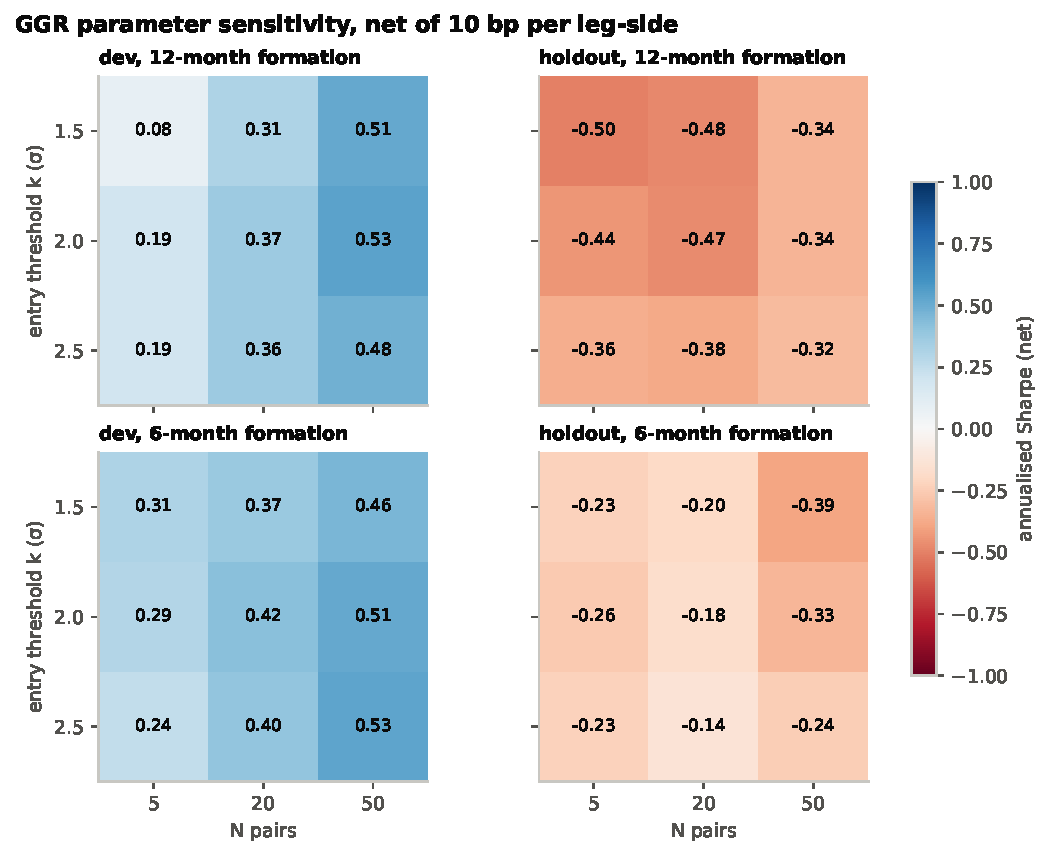
\includegraphics[width=0.62\textwidth]{fig13_sensitivity.pdf}
\caption{Net Sharpe ratios across formation length, entry threshold and number of pairs; development (left) versus holdout (right).}
\label{fig:sens}
\end{figure}

\begin{figure}[t]\centering
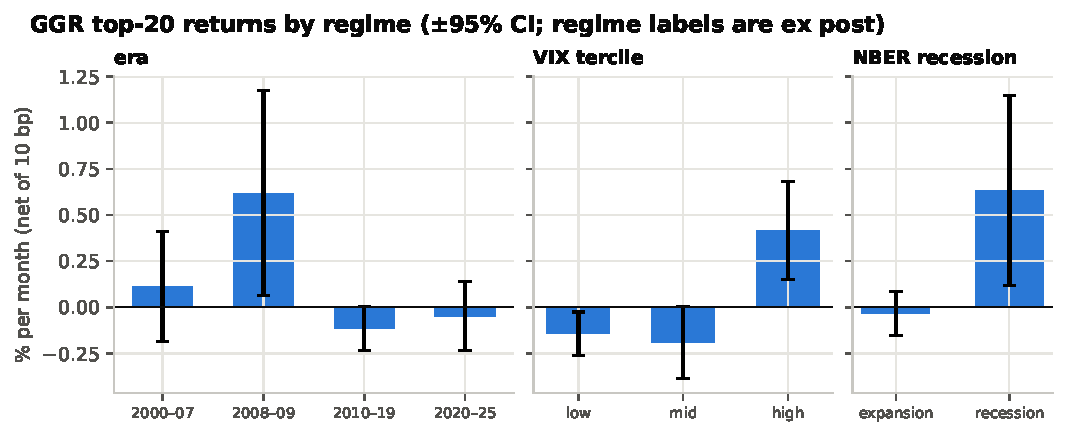
\includegraphics[width=0.85\textwidth]{fig15_regimes.pdf}
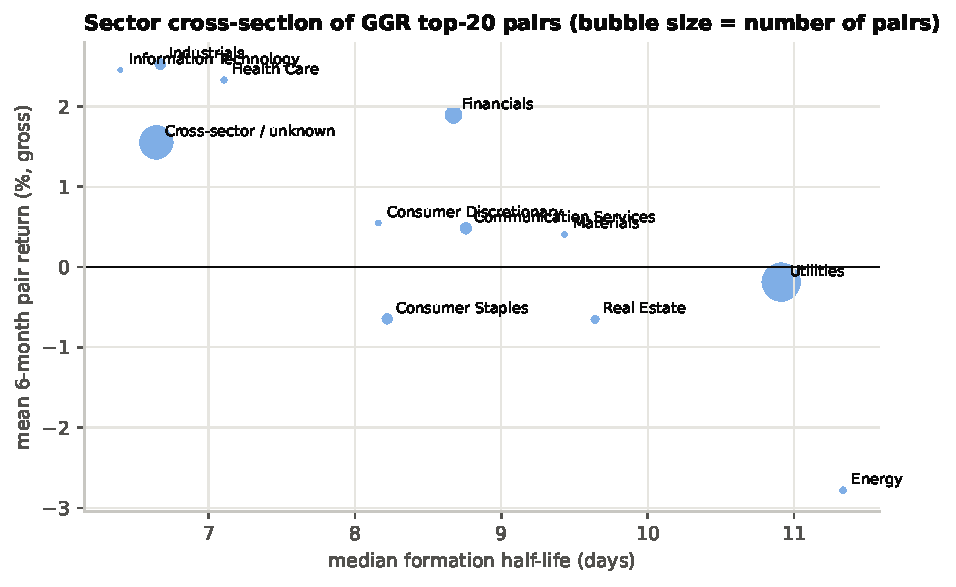
\includegraphics[width=0.6\textwidth]{fig16_sector_crosssection.pdf}
\caption{Top: returns by era, VIX tercile and NBER state ($\pm$95\% CI). Bottom: sector cross-section of top-20 pairs.}
\label{fig:regimes}\label{fig:sector}
\end{figure}

\section{Out-of-Sample Results}

Table~\ref{tab:holdout} reports the formal holdout evaluation (2013--2025). For H2, the Q1$-$Q5 spread with the pre-specified OLS 252-day estimator is 0.36\% per six months ($t=1.04$, $p=0.30$), a fifth of its development value; net of costs it is 0.11\% ($t=0.31$). With the 63-day estimator selected for H5 it is negative ($-0.13\%$). The Fama--MacBeth half-life slope is $-0.0054$ ($t=-1.33$). Half-life persistence (H3) is $\rho=-0.011$. The half-life-filtered portfolio earns $-0.06\%$ per month net (Sharpe $-0.28$) versus $-0.09\%$ for GGR (Sharpe $-0.47$); the difference, 0.04\% per month, is insignificant ($t=1.00$, $p=0.32$). The OU strategy loses 0.31\% per month ($t=-4.57$). After Holm adjustment across the six holdout tests, the smallest adjusted $p$-value is 0.56 (Figure~\ref{fig:holdout}).

\begin{table}[t]\centering\small
\caption{Holdout 2013--2025 (156 months), parameters frozen on 2000--2012. Panel A: hypothesis tests with Holm and Benjamini--Hochberg adjusted $p$-values. Panel B: portfolio performance, monthly.}
\label{tab:holdout}
\begin{tabular}{lrrrr}
\toprule
\multicolumn{5}{l}{\emph{A. Tests}} \\
Hypothesis & Estimate & $p$ & Holm & BH \\
\midrule
H2: Q1$-$Q5, OLS 252d, gross (6-month return) & 0.36\% & 0.300 & 0.910 & 0.318 \\
H2: FM slope on HL rank (controls: SSD rank) & $-0.0054$ & 0.182 & 0.910 & 0.303 \\
H3: Spearman, formation vs realised HL & $-0.011$ & 0.193 & 0.910 & 0.303 \\
H5: HL-filtered minus GGR, net (monthly) & 0.04\% & 0.318 & 0.910 & 0.318 \\
H1/H4: GGR top-20 net mean & $-0.09\%$ & 0.093 & 0.555 & 0.303 \\
H4: HL-filtered net mean & $-0.06\%$ & 0.202 & 0.910 & 0.303 \\
\midrule
\multicolumn{5}{l}{\emph{B. Performance}} \\
Portfolio & Mean (\%/mo) & $t$ & Sharpe & Max DD \\
\midrule
GGR top 20, gross & $-0.00$ & $-0.01$ & $-0.00$ & $-6.2\%$ \\
GGR top 20, net & $-0.09$ & $-1.68$ & $-0.47$ & $-14.2\%$ \\
HL-filtered 20, gross & 0.04 & 0.98 & 0.22 & $-4.1\%$ \\
HL-filtered 20, net & $-0.06$ & $-1.28$ & $-0.28$ & $-10.7\%$ \\
OU (max hold $3\times\HL$), net & $-0.31$ & $-4.57$ & $-1.33$ & $-38.9\%$ \\
\bottomrule
\end{tabular}
\end{table}

\begin{figure}[t]\centering
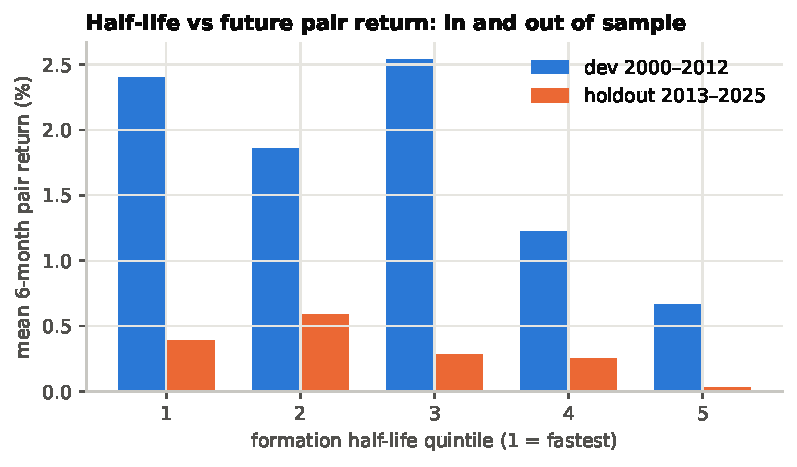
\includegraphics[width=0.49\textwidth]{fig19_h2_dev_vs_holdout.pdf}
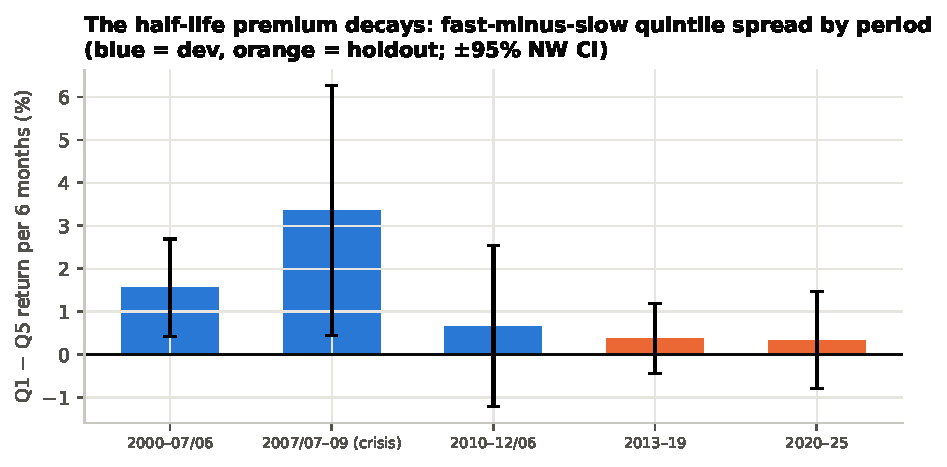
\includegraphics[width=0.49\textwidth]{fig20_h2_subperiods.pdf}
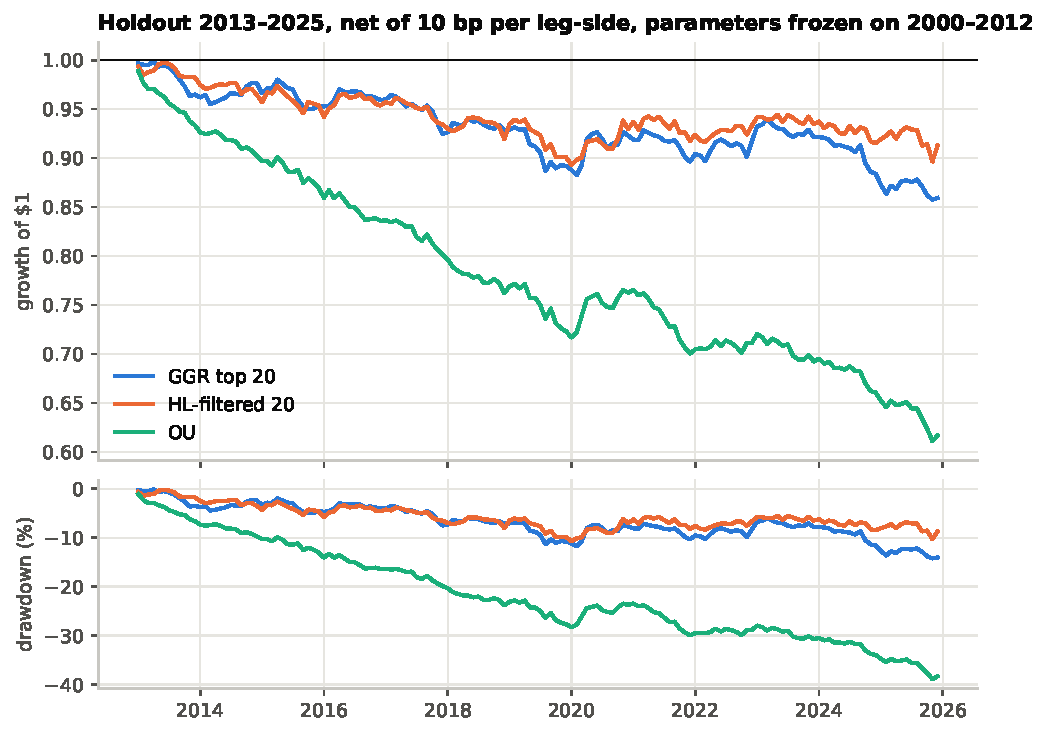
\includegraphics[width=0.75\textwidth]{fig17_holdout_equity.pdf}
\caption{Top left: quintile profiles in and out of sample. Top right: Q1$-$Q5 spread by period. Bottom: holdout equity curves and drawdowns, net of 10 bp.}
\label{fig:holdout}
\end{figure}

\section{Transaction Costs}

Because a top-20 pair completes about 1.5 round trips per six months, each basis point of one-way cost per leg costs about 6~bp per pair per period, or roughly 1~bp per month on committed capital. Figure~\ref{fig:costs} and Table~\ref{tab:breakeven} report break-even costs. In the development sample GGR survives up to 24.5~bp per leg-side, the half-life filter up to 37.8~bp, and the OU rule---which trades far more---up to 11.5~bp. In the holdout the break-even costs are 0, 4.4 and 2.0~bp: below even the most optimistic institutional cost estimates. GGR's own implied cost from the one-day wait was 81~bp of effective spread in their sample; modern large-cap spreads are far lower, but so are the gross profits. H4 is supported in the development sample and rejected in the holdout.

\begin{table}[t]\centering\small
\caption{Break-even transaction cost (bp per leg per side) at which the annualised mean return reaches zero.}
\label{tab:breakeven}
\begin{tabular}{lrr}
\toprule
Strategy & Dev 2000--12 & Holdout 2013--25 \\
\midrule
GGR top 20 & 24.5 & 0.0 \\
Half-life filtered 20 & 37.8 & 4.4 \\
OU, max hold $3\times\HL$ & 11.5 & 2.0 \\
\bottomrule
\end{tabular}
\end{table}

\begin{figure}[t]\centering
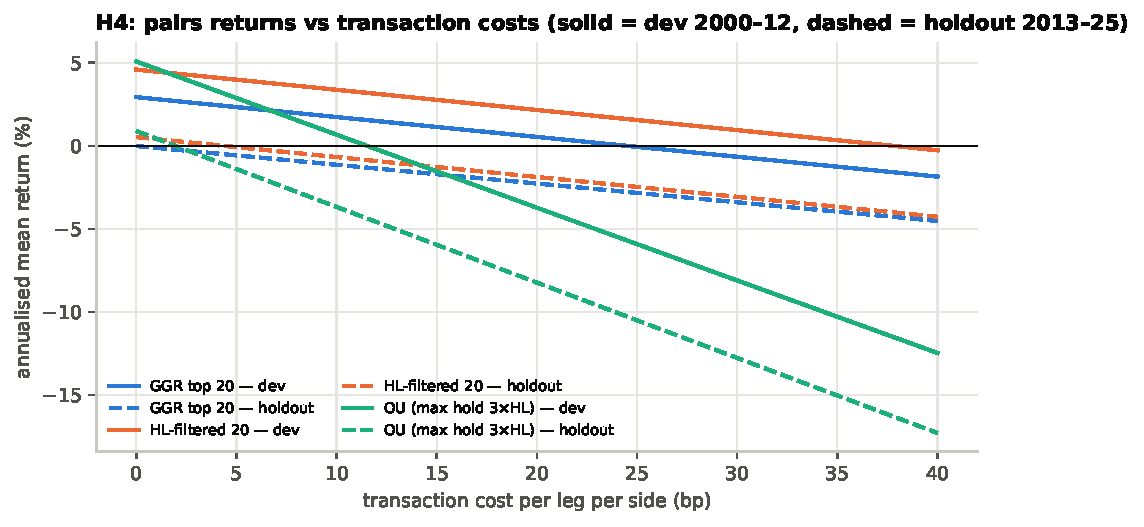
\includegraphics[width=0.85\textwidth]{fig14_cost_sensitivity.pdf}
\caption{Annualised mean return versus cost per leg per side. Solid: development; dashed: holdout.}
\label{fig:costs}
\end{figure}

\section{Economic Interpretation}

Three observations fit together. First, half-life is not a stable pair attribute: its formation estimate predicts the realised half-life essentially not at all. Second, in 2000--2012 it nonetheless predicted returns. Third, the half-life rank is highly correlated with the ADF $p$-value (Spearman 0.83) and the Engle--Granger $p$-value (0.68), but not with the SSD-based trigger width (0.00). A short formation half-life therefore mostly measures how \emph{stationary-looking} the spread was, not how fast it will revert next. Pairs whose spreads oscillated tightly around zero during formation were, in the early 2000s and especially in the 2008--09 crisis, more likely to be linked by a genuine common factor and to reconverge after a liquidity-driven divergence---consistent with GGR's interpretation of pairs profits as compensation for providing liquidity and enforcing the Law of One Price, and with the concentration of profits in high-VIX months. As statistical arbitrage capital grew and large-cap trading costs fell, that compensation shrank for all pairs, and the advantage of fast pairs shrank with it.

Two non-economic explanations must be weighed against this story, and our data cannot fully separate them. The development sample has the worst survivorship coverage (44--68\% of members); if missing firms are disproportionately those whose spreads diverged permanently, the slow-reverting quintile in the observed sample is not representative, and the measured Q1$-$Q5 spread could partly reflect selection. And the development sample is where the strategy, and the half-life signal, were searched for: the deflated Sharpe ratio corrects for the 21 variants we tried, but not for the many prior studies of the same data. The holdout is the only test that is immune to both concerns, and it finds no effect. The correlation evidence is about which pairs earned money; it does not establish that fast reversion \emph{causes} profits.

\section{Limitations}

\begin{itemize}
\item \textbf{Survivorship bias.} Yahoo Finance omits 426 of 1,117 historical members, so coverage rises from 44\% (1999) to 97\% (2025). The bias most likely inflates returns, especially in 2000--2012. A survivorship-free source (CRSP, or a vendor carrying delisted tickers) would be needed to remove it.
\item \textbf{Universe.} Large-cap S\&P~500 stocks only, versus GGR's full CRSP cross-section; average universe 339 stocks.
\item \textbf{Prices.} Adjusted closes approximate total returns; Yahoo adjustments occasionally contain errors; ticker re-use is mitigated, not eliminated, by spell masking and the stale-price screen.
\item \textbf{Sectors.} GICS sectors are current, not point-in-time, and available only for stocks that are still index members today. The sector-restricted portfolio (Table~\ref{tab:replication}) and the same-sector share (Table~\ref{tab:tradestats}) are therefore built only from stocks that survived in the index to 2025 (79\% of the formation universe in 2000, 92\% in 2024)---a use of future information. They are reported for comparison with GGR only; no hypothesis test depends on them.
\item \textbf{Costs.} A linear cost per leg-side; no market impact, no short-borrow fees or recalls, no financing spread on the short proceeds.
\item \textbf{Risk adjustment.} We report raw excess returns; GGR's factor regressions (Fama--French, momentum, reversal) are not replicated.
\item \textbf{Random-pairs baseline.} Uniformly random pairs, not GGR's bootstrap matched on prior-month return deciles.
\item \textbf{Single holdout.} One 13-year holdout is one draw; the effect could reappear in a different regime.
\end{itemize}

This study is a hypothesis test. Neither the replication nor the extension is evidence of a profitable, deployable strategy.

\section{Conclusion}

On point-in-time S\&P~500 data, the GGR distance rule earned modest returns in 2000--2012 and nothing after 2012, extending the decay documented by \citet{dofaff2010}. Mean-reversion half-life---the most intuitive refinement of the rule---predicted pair returns strongly in the development sample with every reasonable estimator, survived costs and a deflated-Sharpe adjustment, and then failed a pre-specified holdout. Estimated half-life is not persistent, it mainly measures how stationary a spread looked during formation, and its predictive content decayed after 2010. The practical lesson is methodological as much as economic: a $t$-statistic of 3.3 on a plausible, theory-motivated signal in 13 years of data is not sufficient evidence, and a strict development/holdout split is what distinguishes a fading anomaly from a tradable one.

\section{Future Research}

\begin{itemize}
\item Repeat the test on survivorship-free CRSP data over 1962--2025, which would also allow a holdout-style test of the half-life effect inside GGR's own sample.
\item Model time-varying reversion speed directly (regime-switching or state-space OU models) instead of a single formation-period estimate.
\item Test whether half-life interacts with liquidity provision: condition on market-wide volatility or funding conditions at formation, which the regime results suggest matter.
\item Replace the linear cost model with spread and impact estimates from intraday data, and include short-borrow costs.
\item Extend to other asset classes (ETFs, futures, international equities), where the decay of equity statistical arbitrage may not apply.
\end{itemize}

\section*{Reproducibility}
All code, the pinned environment (Python~3.13, \texttt{uv.lock}), unit tests, experiment scripts, data provenance and SHA-256 manifest, the frozen-parameter file, and the holdout record (with the commit at which it ran) are in the accompanying repository. Yahoo Finance's terms do not permit redistribution of the price data; the scripts regenerate it.

\bibliographystyle{apalike}
\bibliography{references}

\end{document}
